\chapter{The \BdToKstll decay	}
\label{chap:kstmm:theo}

\section{Angular basis}
\label{sec:kstmm:basis}

The differential angular distribution for \BdToKstll is expressed as a
function of  five kinematic variables: three angles (\ctl, \ctk, $\phi$) 
and two invariant masses;
the mass squared of the \kpi system is denoted \psq and the 
mass squared of the dilepton pair (\qsq),  
the angle $\theta_K$ is defined as the angle between the \Kp and the \B momentum
vector in the rest frame of the \Bd.  The angle $\theta_\ell$ is
 defined as the one between the \ellp in the rest frame of the dilepton
pair and the momentum vector of the \Bd.  The angle $\phi$ is defined
as the signed angle between the planes formed by the dilepton pair and the \kpi pair respectively, 
in the rest frame of the \Bd.\footnote{This is the same sign convention for \ctl as used in all 
previous experiments and the same $\phi$ convention as used in 
\lhcb~\cite{Aaij:2013iag}.}

For the \CP-conjugate decay \BdbToKstbll, $\theta_\ell$ is defined with respect to the \ellm instead of the \ellp
and $\theta_K$ is defined with respect to the \Km instead of the \Kp.
There are two possible definitions of $\phi$, a \CP symmetric definition which 
changes through a minus sign and a \CP anti-symmetric definition, \phiacp, 
which is unchanged between the \Bd and \Bdb decay. 
An illustration of the angles for \BdbToKstbll is shown in Fig~\ref{fig:kstmm:angles}.
\begin{figure}[tbp]
\centering
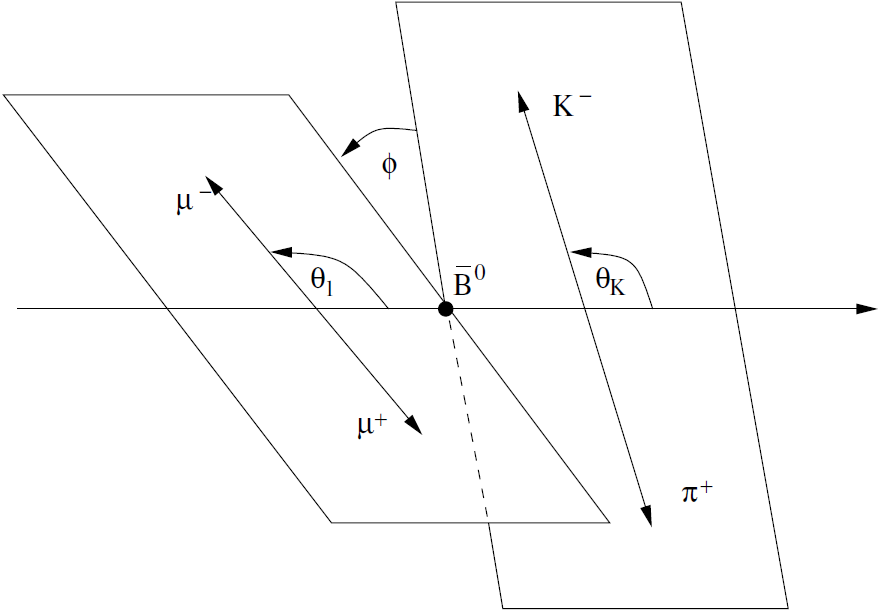
\includegraphics[width=0.48\columnwidth]{chapter4/figs/restMassAngles.png}
\caption[An illustration of the angles used to describe the \BdbToKstbll decay.]
{An illustration of the angles used to describe the \BdbToKstbll decay.
 The angle $\theta_l$ is defined between the \ellm and the \Bdb in the dilepton rest frame.
 The angle $\theta_K$ is defined between the \Km and the \Bdb in the \kpi rest frame.
 The angle $\phi$ is the signed angle between $\ellm$ and $\Km$ in the rest frame of the \Bdb. 
~\label{fig:kstmm:angles} }
\end{figure}

The angles \ctl and \ctk are given explicitly as 
\begin{align}
\ctl = \left( \frac{ \vec{p}_{\ellp} \cdot \vec{p}_{\ellell}  }{|\vec{p}_{\ellp}||\vec{p}_{\ellell}|} \right), \quad 
\ctk = \left( \frac{ \vec{p}_{\Kp} \cdot \vec{p}_{\kpi}  }{|\vec{p}_{\Kp}||\vec{p}_{\kpi}|}  \right) \, ,
\end{align}
where each momentum vector $\vec{p}$ is defined in the rest frame of the parent particle, i.e. 
the lepton momentum, $\vec{p}_{\ellp}$, is in the dilepton rest frame and dilepton momentum, $\vec{p}_{\ellell}$, is in \Bd rest frame.
The angle $\phi$ is calculated as %the difference between the angles $\theta_\ell$ and $\theta_K$ and
\begin{align}
\cos\phi &=    \left( \frac{\vec{p}_{\ellp} \times \vec{p}_{\ellm} }{|\vec{p}_{\ellp} \times \vec{p}_{\ellm}|} \right) \cdot 
   \left( \frac{\vec{p}_{\Kp} \times \vec{p}_{\pim} }{|\vec{p}_{\Kp} \times \vec{p}_{\pim}|} \right)  \, .
\end{align}
%and
%\begin{align}
%\sin\phi =    \left(\frac{ \vec{p}_{\ellp} \times \vec{p}_{\ellm} }{|\vec{p}_{\ellp} \times \vec{p}_{\ellm}|} \right) \times 
%   \left(\frac{ \vec{p}_{\Kp} \times \vec{p}_{\pim} }{|\vec{p}_{\Kp} \times \vec{p}_{\pim}|} \right) 
%   \cdot \frac{\vec{p}_{\kpi}}{|\vec{p}_{\kpi}|}  \, .
%\end{align}
For the CP-conjugate \BdbToKstbll decay, the angles \ctl and \ctk are given explicitly as 
\begin{align}
\cos\theta_{\bar{\ell}} &= \left( \frac{ \vec{p}_{\ellm} \cdot \vec{p}_{\ellell}  }{|\vec{p}_{\ellm}||\vec{p}_{\ellell}|} \right), \quad 
\cos\theta_{\bar{K}} = \left( \frac{ \vec{p}_{\Km} \cdot \vec{p}_{\kpi}  }{|\vec{p}_{\Km}||\vec{p}_{\kpi}|}  \right) \, ,
\end{align}
and applying the \CP operator to the definition of $\phi$ gives the relation,
\begin{align}
\cos\phi &= \left( \frac{\vec{p}_{\ellm} \times \vec{p}_{\ellp} }{|\vec{p}_{\ellm} \times \vec{p}_{\ellp}|} \right) \cdot 
   \left( \frac{\vec{p}_{\Km} \times \vec{p}_{\pip} }{|\vec{p}_{\Km} \times \vec{p}_{\pip}|} \right)  \, . 
\end{align}
The \CP anti-symmetric definition of $\phi$ is given by only applying the \CP operator to the \kpi state, 
\begin{align}
\cos\phiacp &= \left( \frac{\vec{p}_{\ellp} \times \vec{p}_{\ellm} }{|\vec{p}_{\ellp} \times \vec{p}_{\ellm}|} \right) \cdot 
   \left( \frac{\vec{p}_{\Km} \times \vec{p}_{\pip} }{|\vec{p}_{\Km} \times \vec{p}_{\pip}|} \right)  \, .
\end{align}

Each of the angles are defined over the intervals
\begin{align}
0 \leq \theta_{\textit{l}} < \pi, \quad 0 \leq \theta_{\textit{K}} < \pi, \quad -\pi \leq \phi < \pi,
\end{align}
such that the angular distribution is defined over the range
\begin{align}
-1 \leq \ctl < 1, \quad -1 \leq \ctk < 1, \quad -\pi < \phi < \pi \, .
\end{align}

%section
\section{Angular distribution}
\label{sec:fullangdist}

Following Ref~\cite{PhysRevD.61.114028}, the angular distribution of \BdToKstll can be written as an explicit function
of \ctl and $\phi$, 
\begin{align}
\frac{\text{d}^5\Gamma}{\text{d}q^2 \text{d}p^2 \text{d}\ctk \text{d}\ctl \text{d}\phi} = & 
\frac{3}{8} \left( I_1^c + 2I_1^s + (I_2^c + 2I_2^s) \cos2\theta_l  + 2I_3\stlsq\cos2\phi \right. \nonumber \\
&+ 2\sqrt{2}I_4\sin2\theta_l\cos\phi  + 2\sqrt{2}I_5\stl\cos\phi + 2I_6\ctl \nonumber\\ 
&+ \left. 2\sqrt{2}I_7\stl\sin\phi  + 2\sqrt{2}I_8\sin2\theta_l\sin\phi + 2\sqrt{2}I_9\stlsq\sin2\phi \frac{}{} \right) \, ,
\end{align}
where each of the angular coefficients ($I_i$) are combinations of the helicity amplitudes and contain
 an implicit dependence on \ctk and the invariant masses, \psq and \qsq.

The nine angular coefficients are expressed as
\begin{subequations}\begin{align}
I_1^c &= |\mathcal{A}_{0L}|^2 + |\mathcal{A}_{0R}|^2 + 8\frac{m_l^2}{q^2}\Re(\mathcal{A}_{L0}\mathcal{A}_{R0}^{*}) + 4\frac{m_l^2}{q^2}|\mathcal{A}_t|^2 \frac{}{}   \\
I_1^s &= \frac{3}{4} ( |\mathcal{A}_{L||}|^2 + |\mathcal{A}_{L\bot}|^2 + (L\to R) )  ( 1 - \frac{4m_l^2}{q^2} ) +  \frac{4m_l^2}{q^2}\Re( \mathcal{A}_{L\bot} \mathcal{A}_{R\bot}  + \mathcal{A}_{R||} \mathcal{A}_{R||} ) )  \frac{}{} \\
I_2^c &= - \beta_l^2 \left( |\mathcal{A}_{L0}|^2 + |\mathcal{A}_{R0}|^2 \right) \frac{}{} \\
I_2^s &= \frac{1}{4} \beta_l^2 \left( |\mathcal{A}_{L||}|^2 + |\mathcal{A}_{L\bot}|^2 + |\mathcal{A}_{R||}|^2 + |\mathcal{A}_{R\bot}|^2  \right)  \frac{}{} \\
I_3 &= \frac{1}{2} \beta_l^2  \left( |\mathcal{A}_{1L\bot}|^2 - |\mathcal{A}_{1L||}|^2 + |\mathcal{A}_{R\bot}|^2 - |\mathcal{A}_{R||}|^2 \right) \frac{}{}  \\
I_4 &= \frac{1}{\sqrt{2}}   \beta_l^2  \left(  \Re(\mathcal{A}_{L0}\mathcal{A}_{L||}^{*}) + (L\to R) \right) \frac{}{} \\
I_5 &= \sqrt{2}  \beta_l \left(  \Re(\mathcal{A}_{L0}\mathcal{A}_{L\bot}^{*}) - (L\to R) \right) \frac{}{} \\
I_6 &= 2   \beta_l \left( \Re(\mathcal{A}_{L||}\mathcal{A}_{L\bot}^{*}) - (L\to R) \right) \frac{}{} \\
I_7 &= \sqrt{2}  \beta_l \left(  \Im(\mathcal{A}_{L0}\mathcal{A}_{L||}^{*}) - (L\to R) \right) \frac{}{} \\
I_8 &= \frac{1}{\sqrt{2}}  \beta_l^2 \left(  \Im(\mathcal{A}_{L0}\mathcal{A}_{L\bot}^{*}) + (L\to R) \right) \frac{}{} \\
I_9 &=  \beta_l^2 \left(  \Im(\mathcal{A}_{L||}\mathcal{A}_{L\bot}^{*}) + (L\to R) \right) , \frac{}{}
\end{align}\end{subequations}
where $\mathcal{A}_{H(0,||,\bot,t)}$ are the \Kstarz spin amplitudes for a given handedness, $m_l$ is the lepton mass
 and $\beta_l = \sqrt{ 1 - 4m_l^2/\qsq}$~\cite{PhysRevD.61.114028}. 
The lepton mass is assumed to be insignificant, such that $I_{1,2}$ have no $m_l$
dependence, $\beta_l=1$ and $\mathcal{A}_t$ disappears from the angular distribution.

Neglecting any \CP asymmetry, as measured in Ref.~\cite{LHCb-PAPER-2012-021},
%and using $\phi = \phi_{sym}$, 
the \Bd and \Bdb decays can be combined to give 
\begin{align}
\frac{\text{d}^5\left[\Gamma_{\Bd} + \Gamma_{\Bdb} \right] }{\text{d}q^2 \text{d}p^2 \text{d}\ctk \text{d}\ctl \text{d}\phi} = \sum_{i=1}^{9} I_i (\ctl,\ctk,\phi) + \bar{I}_i (\ctl,\ctk,\phi) \ .
\end{align}
The \CP anti-symmetric angular distribution is given by 
\begin{align}
\frac{\text{d}^5\left[\Gamma_{\Bd} - \Gamma_{\Bdb} \right] }{\text{d}q^2 \text{d}p^2 \text{d}\ctk \text{d}\ctl \text{d}\phi} = \sum_{i=1}^{9} I_i (\ctl,\ctk,\phi) - \bar{I}_i (\ctl,\ctk,\phiacp) \ .
\end{align}
Simplification of the angular distribution can be achieved by applying a transformation 
 in $\phi$ such that $\phiprime = \phi - \pi $ 
for $\phi < 0 $~\cite{Ksteepubnote}.
The $I_{4,5,7,8}$ angular terms which are dependent on $\cos\phi$ or
$\sin\phi$ cancel, leaving $I_{1,2,3,6,9}$ in the angular distribution.

For a \kpi state which is a combination of different resonances,
the amplitudes for a given handedness ($H=L,R$) can be expressed as a
sum over the resonances ($J$)~\cite{Lu:2011jm},
\begin{equation}
\label{eq:amp}
\begin{aligned}
\mathcal{A}_{H,0/t}^{L,R}(\psq,\qsq) &= \sum_J \sqrt{N_J} \ A_{J,H,0}^{L,R}(\qsq) \ P_J(p^2) \ Y_J^0 (\theta_K,0)  \\
\mathcal{A}_{H,||/\bot}^{L,R}(\psq,\qsq) &= \sum_J \sqrt{N_J} \ A_{J,H,||/\bot}^{L,R}(\qsq) \ P_J(p^2) \ Y_J^{-1} (\theta_K,0) , 
\end{aligned}
\end{equation}
where $Y_J^m (\theta_K, 0)$ are the spherical harmonics, $\mathcal{M}$
is the matrix element encompassing the \qsq dependence
 and $P_J(\psq)$ is the propagator of the resonant \Kstarz state.




%section
\section{Amplitudes}
\label{sec:kstmm:amps}

The amplitudes of \BdToKpill parametrise the decay and are different for each polarisation of the \kpi state and of the dilepton system.
The dilepton is a vector state and the \kpi system is considered to be in a scalar (S-wave) or a vector (P-wave) state.
The matrix element for  \BdToKpill takes the same form for  both \kpi states and can be written~\cite{AltmannshoferBall} as
\begin{align}
\mathcal{M} =& \frac{G_F \alpha_s}{2\pi} \Vtb\Vts \bigg( \bigg[ \bra\kpi  \bar{s}\gamma_\mu \left( \Ceff9 P_L + \Cpeff9 P_R \right) \bquark \ket{\bar{B}}  \nonumber \\
 &  - \frac{2m_b}{\qsq} \bra\kpi  \bar{s} i \sigma^{\mu\nu} q_\nu \left( \Ceff7 P_R + \Cpeff7 P_L \right) \bquark\ket{\bar{B}} \bigg] \left( \bar{\ell}\gamma_{\mu} \ell\right)  \nonumber \\
 &  + \bra\kpi  \bar{s} \gamma^\mu \left( \Ceff10 P_L + \Cpeff10 P_R \right) b \ket{\bar{B}} \left( \bar{\ell} \gamma_\mu \gamma_5 \ell \right)   \bigg)    
\end{align}
where contributions from scalar and pseudoscalar operators have been ignored.

\subsection{\BdToKstll}

The \kpi P-wave has three polarisation states:
The total amplitude for the decay of a pseudo-scalar to two vector particles, $\decay{P}{V_1 V_2}$, can be written as a combination of the 
polarisation tensors and the matrix element,
\begin{align}
\label{eq:pol}
M(\decay{P}{V_1 V_2}) &= \epsilon_{V_1}^{*\mu} M_{\mu\nu} \epsilon_{V_2}^{*\nu} \, .
\end{align}
Each of the polarisation states for a vector state described by the momentum vector 
$p^\mu = \left(p_0, 0, 0, p_z\right)$ can be written as
\begin{subequations}\begin{align}
\epsilon_V^\mu(\pm) &= \left( 0, 1, \pm i, 0\right) / \sqrt{2} \\
\epsilon_V^\mu(0) &= \left( p_z, 0, 0, -p_0\right) / \sqrt{p^2} \\
\epsilon_V^\mu(t) &= \left( p_0, 0, 0, p_z\right) / \sqrt{p^2} \ .
\end{align}\end{subequations}
In the context of the decay \BdToKstll there is a virtual gauge boson and a real \Kstarz.
The gauge boson can exist in all four possible polarisation states $(0, \pm, t)$ but the \Kstarz is on shell and only 
 has three states $(0, \pm)$.
The helicity amplitudes can be obtained by contracting the polarisation states for each of the 
particles in Eq~\ref{eq:pol} to give 
\begin{align}
H_i = M_{i,i} \, ,
\end{align}
with an implicit sum over $i = 0, ||$ and $\bot$, and additionally $H_t = M_{0,t}$.
The transversity amplitudes are combinations of the helicity amplitudes
\begin{align}
A_{||,\bot} = ( H_{+} \mp H_{-} ) \sqrt{2} , \quad A_0 = H_0 , \quad \text{and} \,  A_t = H_t 
\end{align}
The subsequent decay of the vector boson to dilepton system allows for both left and right-handed currents in 
the longitudinal, parallel and perpendicular polarisations so there are in total seven transversity amplitudes.
The transversity amplitudes  for the P-wave \Kstarzo state can be written to leading order~\cite{AltmannshoferBall} as	
\begin{subequations}\begin{align}
A_{1,L/R,0}(\qsq)=& -\frac{N}{2m_{\Kstarzo}\sqrt{\qsq}} \Bigg(  \left( (\Ceff9 - \Cpeff9 ) \mp (\Ceff10 - \Cpeff10 ) \right)  \nonumber\\ 
 & \bigg[ \left( \mB^2 - m_{\Kstarzo}^2 - \qsq \right) \left( \mB + m_{\Kstarzo} \right) A_1(\qsq) - \lambda \frac{A_2(\qsq)}{\mB + \m_{\Kstarzo}} \bigg]   \\ 
 & + 2m_b \left( \Ceff7 - \Cpeff7 \right) \bigg[ \left( \mB^2 + 3m_{\Kstarzo}^2 + \qsq \right) T_2(\qsq) - \frac{\lambda(\mB,\Kstarzo,\qsq)}{\mB^2 - m^2_{\Kstarzo}} T_3(\qsq) \bigg] \Bigg) \nonumber \\
A_{1,L/R,||}(\qsq) =& -N \sqrt{2}\left(\mB^2 - m_{\Kstarzo}^2\right) \bigg[ \left( (\Ceff9 - \Cpeff9 ) \mp (\Ceff10 - \Cpeff10 ) \right) \frac{ A_1(\qsq) }{ \mB + m_{\Kstarzo} } \nonumber \\
& + 2\frac{m_b}{\qsq} \left( \Ceff7 - \Cpeff7 \right) T_ 2(\qsq) \bigg] \\
A_{1,L/R,\bot}(\qsq) =&  N \sqrt{2} \lambda(\mB,\Kstarzo,\qsq)^{1/2}  \bigg[ \left( (\Ceff9 - \Cpeff9 ) \mp (\Ceff10 - \Cpeff10 ) \right) \frac{ V(\qsq) }{ \mB + m_{\Kstarzo} } \nonumber \\
& + 2\frac{m_b}{\qsq} \left( \Ceff7 + \Cpeff7 \right) T_1(\qsq) \bigg] 
\end{align}\end{subequations}
with $\lambda(\mB,\psq,\qsq) = \left( \mB^2 - \psq - \qsq \right)^2 - 4\psq\qsq$.
This expression uses the narrow width assumption for the \Kstarz(892) which assumes the \Kstarz decays on shell to \kpi, 
 allowing the relativistic Breit-Wigner to be approximated as
\begin{align}
P_1^2(\psq) = \frac{1}{\left(\psq + m_{\Kstarz}^2\right)^2 +m_{\Kstarz}^2 \Gamma_{m_{\Kstarz}}^2 }   \frac{m_{\Kstarz}\Gamma_{m_{\Kstarz}}}{\pi}  \quad \to   \quad  \delta\left(\psq-m_{\Kstarz}^2\right) \ .
\end{align}
The transversity amplitudes can then be expressed in terms of seven \B\to\Kstarzo form factors ($A_i(\qsq), T_i(\qsq), V(\qsq)$).
For large \Kstar energies, of order $\mB/2$, it is possible to reduce the seven different 
form factors to two \emph{heavy-to-light} form factors as in Ref~\cite{Kruger:2005ep}.
This allows the amplitudes to take a simple form neglecting corrections of order $1/m_b$ and $\alpha_S$,
\begin{subequations}\begin{align}
A_{1,L/R,0}(\qsq)=& -\frac{N}{2m_{\Kstarzo}\sqrt{\qsq}} (1-\qsq)^2 \Bigg[  \left( (\Ceff9 - \Cpeff9 ) \mp (\Ceff10 - \Cpeff10 ) \right) \nonumber\\
&+ 2m_b \left( \Ceff7 - \Cpeff7 \right) \Bigg]  \xi_{||}\left(E_{\Kstarz}\right)   \\
A_{1,L/R,||}(\qsq) =& -N \sqrt{2}\mB (1-\qsq) \bigg[ \left( (\Ceff9 - \Cpeff9 ) \mp (\Ceff10 - \Cpeff10 ) \right) \nonumber\\ 
& + 2\frac{m_b}{\qsq} \left( \Ceff7 - \Cpeff7 \right) \bigg] \xi_{\bot}\left(E_{\Kstarz}\right) \\
A_{1,L/R,\bot}(\qsq) =& + N \sqrt{2}  \mB (1-\qsq) \bigg[ \left( (\Ceff9 - \Cpeff9 ) \mp (\Ceff10 - \Cpeff10 ) \right) \nonumber \\
& + 2\frac{m_b}{\qsq} \left( \Ceff7 + \Cpeff7 \right)  \bigg] \xi_{\bot}\left(E_{\Kstarz}\right) \, .
\end{align}\end{subequations}

\subsection{\BdToKpill amplitudes}

Non-resonant \kpi effects in have been explored in Ref~\cite{Grinstein:2005ud} and the combination of multiple
 \Kstar resonances have been explored in Ref~\cite{Lu:2011jm}.
A combination of several resonant \kpi states can be achieved though the dependence
of the matrix elements on the resonant mass, $m_{\Kstarzj}$ 
and adding coefficients derived from the polarisation tensor~\cite{Lu:2011jm}.
The effect of a \kpi S-wave has been explored in Refs~\cite{Becirevic:2012dp,Matias:2012qz} and also in more detail later in Chapter~\ref{chap:swave:theo}.
The single \Kstarzz S-wave amplitude~\cite{Lu:2011jm} is given by
\begin{align}
A_{0,L/R,0} =& N\frac{\lambda\left(\mB,\Kstarzz\qsq\right)^{1/2}}{\sqrt{\qsq}} \bigg[ \left( (\Ceff9 - \Cpeff9 ) \mp (\Ceff10 - \Cpeff10 ) \right) F_1(\qsq)  \nonumber \\
&+ 2 m_b \left( \Ceff7 + \Cpeff7 \right) \frac{ F_T(\qsq)}{\mB + m_{\Kstarzz} }  \bigg]  
\end{align}
where $F_1(\qsq)$ and $F_T(\qsq)$ are the \Bd\to\Kstarzz form factors. 





%section
\section{Angular observables}
\label{sec:kstmm:obs}

The contributions from the Wilson coefficients defined above
 can be measured by measuring the transversity amplitudes
 through an angular analysis of the \BdToKstll angular distribution.
Direct measurements of the transversity amplitudes are dependent on the values of the form factors
 which have a significant theoretical uncertainty.
To mitigate these uncertainties and allow measurements of the Wilson coefficients, angular observables
can be constructed from the transversity amplitudes that are independent of the two heavy-to-light form factors.
Many angular observables have been proposed for the decay 
\BdToKstll~\cite{Kruger:2005ep,AltmannshoferBall,Egede:2008uy,Bobeth:2010wg,Matias:2012xw}. 
These observables are combinations of the amplitudes which both minimise the uncertainty from the form factors 
and maximise the contribution from new physics models. 
So far the forward-backward asymmetry (\AFB), the fraction of the \Kstarz longitudinal polarisation (\FL ) 
and two combinations of the transverse amplitudes (\AT2 and \AIm ) have been 
measured~\cite{Aaltonen:2011cn,Aubert:2007hz,Aaltonen:2011ja,Aubert:2008ju,PhysRevLett.103.171801}.

\subsection{P-wave observables}

These observables are constructed from combinations of amplitudes and
are normalised to the sum of amplitudes for the P-wave state, given as 
\begin{align}
|A_{10}|^2 + |A_{1||}|^2 + |A_{1\bot}|^2 \, ,
\end{align}
where the generic combination of amplitudes $A_{Ji}A_{Ji}^{*}$ is defined for a spin $J$ and a polarisation (0,$||$,$\bot$) as
\begin{align}
\label{eq:ampsq}
A_{Ji} A_{Ji}^{*} &= A_{JiL} A_{JiL}^{*} + A_{JiR} A_{JiR}^{*} \, .
\end{align}
The forward-backward asymmetry of the dilepton system, \AFB, enters in the angular coefficient $I_6$ and
is defined in terms of the amplitudes as
\begin{align}
\label{eq:theoafb}
\AFB(\qsq) &= \frac{3}{2} \frac{  \Re(A_{1L||}A_{1L\bot}^{*}) - 
\Re(A_{1R||}A_{1R\bot}^{*})}{|A_{10}|^2 + |A_{1||}|^2 + |A_{1\bot}|^2 } \, .
\end{align}
In a similar way, \FL, \OS3 and \OS9 are defined as
\begin{equation}
\begin{split}
\FL(\qsq) &= \frac{  |A_{10}|^2 } {|A_{10}|^2 + |A_{1||}|^2 + |A_{1\bot}|^2} \\
\OS3 (\qsq) &= \frac{ |A_{1\bot}|^2 - |A_{1||}|^2 }{ |A_{10}|^2 + |A_{1||}|^2 + |A_{1\bot}|^2} \\
\OS9 (\qsq) &= \frac{  \Im(A_{1L||}A_{1L\bot}^{*}) - \Im(A_{1R||}A_{1R\bot}^{*}) }{|A_{10}|^2 + |A_{1||}|^2 + |A_{1\bot}|^2} 
\end{split}
\end{equation}
where \OS3 and \OS9 are related to the angular coefficients $I_3$ and $I_9$ respectively.
These theoretical observables are normalised to the sum of the P-wave amplitudes
and the factorisation of the amplitudes into matrix elements and the 
propagators removes the \psq dependence from these theoretical observables. 

In terms of the angular distribution, \AFB can also be expressed 
as the difference 
between the number of `forward-going' \mup and the number of 
`backward-going' \mup in the rest frame of the \Bd,
\begin{align}
\label{eq:expafb}
\left[ \int_0^1 - \int_{-1}^0 \right]  \text{d}\ctl
\frac{\text{d}\Gamma}{\text{d}\qsq \text{d}\ctl} / 
\frac{\text{d}\Gamma}{\text{d}\qsq} \, ,
\end{align}
which explains the name of the observable. 

\subsection{Transverse observables}
\label{sec:kstmm:reparam}

Angular observables which are normalised to only the transverse helicity amplitudes have
 been studied with the additional aim of reducing the theoretical uncertainties~\cite{Melikhov:1998cd,Kruger:2005ep}.
This is achieved by separating out the dependence on the  longitudinal amplitudes and their form factors from the calculation.
The main transverse observable is \AT2 which comes from the angular coefficient $I_3$,
\begin{align}
\AT2 (\qsq) &=  \frac{ |A_{1\bot}|^2 - |A_{1||}|^2  }{ |A_{1\bot}|^2 + |A_{1||}|^2 }  \, .
\end{align}
The observables associated with $I_6$ and $I_9$ can be similarly reparameterised~\cite{Becirevic:2011bp} 
 to give
\begin{equation}
\begin{split}
\ATRe(\qsq) &= \frac{ |A_{1\bot}|^2 - |A_{1||}|^2 }{ |A_{1||}|^2 + |A_{1\bot}|^2} \\
\ATIm(\qsq) &= \frac{  \Im(A_{1L||}A_{1L\bot}^{*}) \Im(A_{1R||}A_{1R\bot}^{*}) }{ |A_{1||}|^2 + |A_{1\bot}|^2} \, .
\end{split}
\end{equation}
These observables are correlated to $(1-\FL)$ when the the angular distribution is normalised to the sum of the P-wave amplitudes.

\subsection{\CP asymmetric angular observables}

Angular observables equivalent to \OS3 and \OS9 for the \CP antisymmetric angular distribution can by constructed
from the definition of $I_i - \bar{I}_i$.
Two \CP antisymmetric angular observables, \OA3 and \OA9 for the angular coefficients $I_3$ and $I_9$,
which can be compared to the \OS{i} angular observables 
\begin{align}
\OA3 &= \frac{1}{2} \frac{\left(I_3 - \bar{I}_3\right)}{ |A_{10}|^2 + |A_{1||}|^2 + |A_{1\bot}|^2} \, , \\
\OA9 &= \frac{1}{2} \frac{\left(I_9 - \bar{I}_9\right)}{ |A_{10}|^2 + |A_{1||}|^2 + |A_{1\bot}|^2}  \, .
\end{align}

\subsection{Relation to the Wilson coefficients}

Each of the observables is related to the Wilson coefficients through bi-linear combinations of the transversity amplitudes.
This means that there are terms proportional to the combinations $|\Ceff{9,10} \pm \Cpeff{9,10} |^2$ and $|\Ceff7 - \Cpeff7 |^2$.
Each of these terms is multiplied by the relevant \Kstarz form factors giving the \qsq dependence. 
This can be seen in the SM predictions for \AFB and \FL in Fig.~\ref{fig:otherexp}.






%section
\section{The angular distribution with observables}
\label{sec:kstmm:angdistswithobs}

The angular distribution of \BdToKstmm including the angular observables as a function of \ctl, \ctk and \phiprime is given by
\begin{align}
\label{eq:kstmm:theo5d}
\frac{1}{\Gamma} \frac{\text{d}^4\Gamma}{\text{d}\qsq\dctk\dctl \text{d}\phiprime} & =   \frac{9}{16\pi}   \Bigg(  \xspace 2 \FL \ctksq ( 1 - \ctlsq )  \nonumber \\ 
&  \quad \quad \quad  + \frac{1}{2} ( 1 - \FL ) ( 1 - \ctksq ) ( 1 + \ctlsq )  \nonumber \\
&  \quad \quad \quad  + \frac{1}{2} ( 1 - \FL ) \AT2 ( 1 - \ctksq ) (  1 - \ctlsq ) \cos2\phiprime  \nonumber \\
&  \quad \quad \quad  +  \frac{4}{3} \AFB ( 1 - \ctksq ) \ctl  \nonumber \\ 
&  \quad \quad \quad  + \OS{3} ( 1 - \ctksq ) ( 1 - \ctlsq) \sin2\phiprime  \Bigg) . 
\end{align}
The two-dimensional angular distribution as a function of \ctl  and \ctk is given by integrating over $\phi$ in Eq.~\ref{eq:kstmm:theo5d}
\begin{equation}
\label{eq:kstmm:theo4d}
\begin{split}
\frac{1}{\Gamma} \frac{\text{d}^3\Gamma}{\text{d}\qsq\text{d}\ctk \text{d}\ctl} & =   \frac{9}{16} \Bigg( 2 \FL \ctksq ( 1 - \ctlsq )   +\frac{1}{2}  ( 1 - \FL ) ( 1 - \ctksq ) ( 1 + \ctlsq )  \\
& \quad \ + \frac{4}{3} \AFB ( 1 - \ctksq ) \ctl     \Bigg) 
\end{split}
\end{equation}
and further integration from Equation~\ref{eq:kstmm:theo5d} yields the angular distribution for each of the angles,
\begin{equation}
\label{eq:kstmm:theo3d}
\begin{split}
\frac{1}{\Gamma} \frac{\text{d}^2\Gamma}{\text{d}\qsq\dctl} &=   \frac{3}{4} \FL ( 1 - \ctlsq )  + \frac{3}{8} ( 1 - \FL ) ( 1 + \ctlsq ) + \AFB \ctl  , \\
\frac{1}{\Gamma} \frac{\text{d}^2\Gamma}{\text{d}\qsq\dctk}  &=    \frac{3}{2}  \FL \ctksq +  \frac{3}{4} ( 1 - \FL ) ( 1 - \ctksq ) 	, \\
\frac{1}{\Gamma} \frac{\text{d}^2\Gamma}{\text{d}\qsq\text{d}\phiprime } &=   \FL + \frac{1}{2} ( 1 - \FL ) \AT2  \cos2\phiprime +  \OS{3}  \sin2\phiprime  .
\end{split}
\end{equation}
There is a physical limit on the size of \AFB and \FL given by $ \AFB \leq \frac{3}{4} (1-\FL) $, where if $\FL \to 1$, then the parallel and perpendicular amplitudes must tend to zero, implying $\AFB\to0$.

\section{Summary}

In this chapter the angular distribution of \BdToKstll was presented.
The helicity amplitudes for $\Bd\to\Kstarzo\ellell$ and $\Bd\to\Kstarzz\ellell$ are detailed 
 showing the structure arising from a Hamiltonian written in terms of Wilson coefficients.
Several experimental observables are set out which are favoured theoretically for
 the ability to calculate predictions cleanly.

 
